\documentclass{beamer}

%\usepackage{multimedia}

% For more themes, color themes and font themes, see:
% http://deic.uab.es/~iblanes/beamer_gallery/index_by_theme.html
%
\mode<presentation>
{
  \usetheme{Madrid}       % or try default, Darmstadt, Warsaw, ...
  \usecolortheme{seagull} % or try albatross, beaver, crane, ...
  \usefonttheme{serif}    % or try default, structurebold, ...
  \setbeamertemplate{navigation symbols}{}
  \setbeamertemplate{caption}[numbered]
	\setbeamertemplate{footline}{}
	\setbeamersize{text margin right=2pt}
} 

\usepackage{tikz}
\usetikzlibrary{decorations.markings,angles}
\usepackage{tikz-3dplot} 

\usepackage{amsmath}


\begin{document}
%%%%%%%%%%%%%%%%%%%%%%%%%%%%%%%%%%%%%%%%%
\begin{frame}{Corona in visible light}

\begin{itemize}
\item F corona: light scattered by interplanetary dust particles 
\begin{itemize}
\item unpolarized (within 5-6 $R_{Sun}$)
\item  nearly constant in time and unaffected by CME
\item with absorption lines
\end{itemize}
\item K corona: light scattered by electrons in the corona - Thomson scattering 
\begin{itemize}
\item polarized radial (CME?) and tangetial (electrons along magnetic loops?) to the solar limb
\item no absorption lines because of high temperatures
\end{itemize}

\end{itemize}

The brightness of the K corona falls off much more
rapidly with distance from the Sun such that it dominates close to
the Sun, is roughly equal to the F corona at $\approx$ 4 $R_{Sun}$, and is much
dimmer than the F corona far from the Sun. 


\end{frame}

%%%%%%%%%%%%%%%%%%%%%%%%%%%%%%%%%%%%%%%%%


\begin{frame}{Comparison with LASCO observations}

\begin{itemize}
\item close to the sun the light is scattered mostly in the plane of sky
\item use coronagraph with large field of view LASCO (located on SOHO  spacecraft, no atmospehric scattering) for  C2 up to 6 $R_{Sun}$ and C3 up to 32 $R_{Sun}$
\item  synthetic images created by numerically
integrating the Thomson-scattered light along a LOS ($\impliedby$ oplically thin corona) for each
pixel with the appropriate scattering function
\item make truly quantitative comparisons with the data
\item account for F corona far
from the Sun, where it is the dominant source of scattered light
\item the contribution of dust scattering with the
same power-law empirical relationship used to make the LASCO
images. In this case, the background F corona brightness is taken
to have the form: $B_F = c r^{0.22 cos(2\theta) - 2.47} $. 
$c = \{c \mid B_F(r = 4 R_{Sun}) = B_k  \}$,where  $B_K$ is the background polar brightness of
the K corona.

\end{itemize}

\end{frame}

%%%%%%%%%%%%%%%%%%%%%%%%%%%%%%%%%%%%%%%%%
\begin{frame}{Velocity comparison}
\begin{figure}[H]
 \centering
 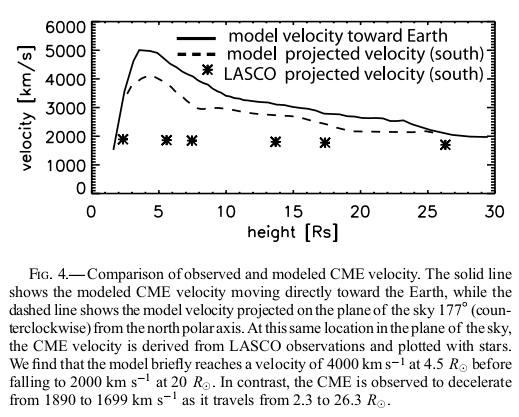
\includegraphics[scale=0.55]{velComp.png}
\end{figure}

\end{frame}
%%%%%%%%%%%%%%%%%%%%%%%%%%%%%%%%%%%%%%%%%

\begin{frame}{Comparison of observed (left) and simulated (right) Thomson-scattered white-light brightness}
\begin{figure}[H]
 \centering
 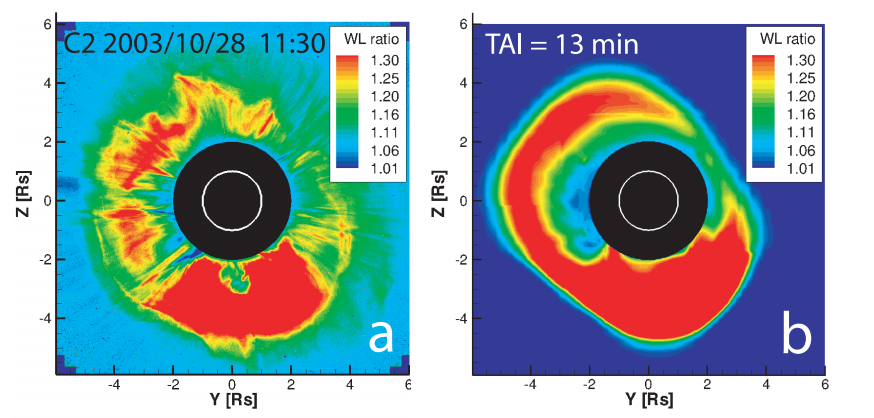
\includegraphics[scale=0.4]{wltime1.png}
\end{figure}

\end{frame}

%%%%%%%%%%%%%%%%%%%%%%%%%%%%%%%%%%%%%%%%%

\begin{frame}{Comparison of observed (left) and simulated (right) Thomson-scattered white-light brightness}
\begin{figure}[H]
 \centering
 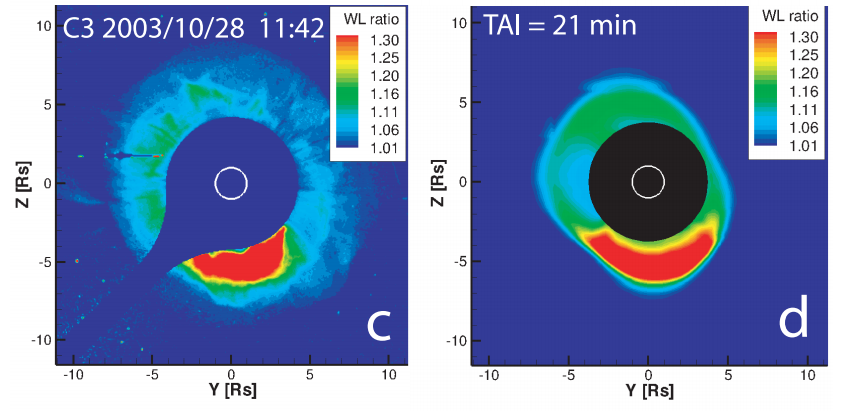
\includegraphics[scale=0.4]{wltime2.png}
\end{figure}

\end{frame}

%%%%%%%%%%%%%%%%%%%%%%%%%%%%%%%%%%%%%%%%%

\begin{frame}{Comparison of observed (left) and simulated (right) Thomson-scattered white-light brightness}
\begin{figure}[H]
 \centering
 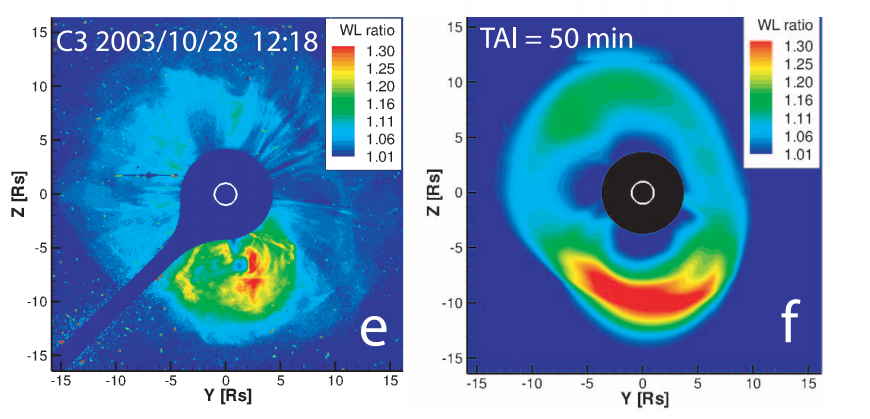
\includegraphics[scale=0.4]{wltime3.png}
\end{figure}

\end{frame}


%%%%%%%%%%%%%%%%%%%%%%%%%%%%%%%%%%%%%%%%%
\begin{frame}{Observations}
\begin{itemize}
\item the CME travels slower than in the model, with
the observed sequence of images occurring at approximately 36,
48, and 84 minutes after initiation. The velocity in the model also larger than in observation.
\item In both data and model, the
color images show the total brightness divided by that of the preevent
background.  
\item White circles show the solar limb, and filled
black circles show the occulting disks.
\item In all cases there is  extremely
good quantitative agreement in both the magnitude and spatial distribution
of the observed brightness.
\item brightest SE, dimmest NW ($\impliedby$  position of AR, which was
located at 20 below the equator on October 28)
\item at 12:18 UT (the third), the
observed brightness patterns is more highly structured than the
model.
\end{itemize}
\end{frame}
%%%%%%%%%%%%%%%%%%%%%%%%%%%%%%%%%%%%%%%%%
\begin{frame}[allowframebreaks]{CME mass}

{\fontsize{10}{12}\selectfont
\begin{itemize}
\item calculated from observations by integrating the excess brightness of the K corona with
the assumption that the plasma is in the plane of the sky, which
sets a lower limit on CME mass. The F corona is subtracted out
from the observations and does not affect the mass. We restrict
this integral to the brightest portion of the CME that extends from
235$^\circ$ to 330$^\circ$ as measured from the  y=0 axis. In the case
of the C2 field of view (top row), this integration sector
extends from 2.0 to 6.0 $R_{Sun}$, and for the C3 field of view (middle and bottom rows) 
the sector extends from 4.0 to 16.4 $R_{Sun}$. 
\item masses derived from observations
 are $1.5\times10^{16}$,$1.55\times10^{16}$ ,and $1.70\times10^{16}$  g, respectively. 
The corresponding masses of the
model CME  are, respectively,  $2.23\times10^{16}$, $2.16\times10^{16}$ $4.90\times10^{16}$ g.
\item The observed masses are approximately 30\% less than that of
the model at times  11:30 and 11:42 UT (first two), which is consistent
with the larger filling factor of the model event. 
\item The slight decrease
in model CME mass found from Figure 5d (second) is the result of a greater
part of the CME being obscured by the occulting disk. 
\item By 12:18  (the third) the CME mass is observed to increase by 13\%, while the model
mass (as shown in Fig. 5f ) more than doubles.
CME mass increases faster than what is observed because of the
excess speed of the CME. For the observed event, the (excess)
mass continues to increase by almost an order of magnitude, to
$13.6\times10^{16}$  g as measured with SMEI on October 29, 12:00 UT,
as the CME passed the Earth.
\item In the numerical model mass increase in the case of the  
fast CMEs as plasma is swept up as they travel from
the Sun, as shown in other numerical simulations is expected.
\item The mass increase seen in
LASCO observations is attributed to mass entering the coronagraph
field of view from below the occulter. In
general, there is not yet proof of a plasma pileup in the low corona
by CMEs. 
\end{itemize}
}
\end{frame}
%%%%%%%%%%%%%%%%%%%%%%%%%%%%%%%%%%%%%%%%%
%%%%%%%%%%%%%%%%%%%%%%%%%%%%%%%%%%%%%%%%%
%%%%%%%%%%%%%%%%%%%%%%%%%%%%%%%%%%%%%%%%%
%%%%%%%%%%%%%%%%%%%%%%%%%%%%%%%%%%%%%%%%%
%%%%%%%%%%%%%%%%%%%%%%%%%%%%%%%%%%%%%%%%%
%%%%%%%%%%%%%%%%%%%%%%%%%%%%%%%%%%%%%%%%%
%%%%%%%%%%%%%%%%%%%%%%%%%%%%%%%%%%%%%%%%%

%\begin{frame}{}
%\begin{itemize}
%\item 
%\end{itemize}
%\end{frame}
\end{document}
